
\begin{appendices}

\renewcommand\thefigure{\thesection.\arabic{figure}}

\appendix
\section{Compiling Flexi and Hopr}\label{Asec:compile}

\begin{enumerate}
 \item Build Flexi: The following steps assume a Linux operating system running bash.
 \begin{itemize}
 \item Be careful to read the README.md and INSTALL.md files to be sure the dependent libraries are available to the compiler/linker.  In particular, be sure the ``libopenmp-dev'' /library is installed and available for both Flexi and Hopr.
  \item In the directory where you want the source code for Flexi to reside type: git clone \url{https://github.com/flexi-framework/flexi.git} (or else download the ZIP file).
  \item Change directories to the new flexi-directory just created by ''git``. In that top-level Flexi directory, make a new directory called ''build`` and change directory to that directory. Create a new text file (shell script) called, for example, ''do-config`` (using the cases in \ref{sec:configFiles} as examples or by following the Flexi Project Documentation guidance) including the first line: ''\#!/bin/sh`` and the last lines ''$\backslash$" and ``..'' as shown. The flags given there are those needed to compute the compressible flow results given above. Save the file and, since it is a bash-script type: ``chmod u+x do-config'' so it can be executed.  Then, type: ``./do-config'', which runs cmake on the proper files.  (Check the github Flexi site for a complete description of how to build the code as well as any needed dependancies to be sure your computer has all the libraries needed; particularly all the ``mpi'' libraries.)
  \item With successful completion of the prior step, then simply type: ``make'' to build the code.  The executables will reside in the build directory. Note that during the compile step, hdf5-files may be downloaded and compiled (ignore the many compile warnings) if a system wide hdf5-library cannot be found by cmake.
 \end{itemize}
\item Build Hopr: Hopr is a mesh generation code available using: ``git clone \url{https://github.com/flexi-framework/hopr.git}''.  It generates a \.h5 mesh file using a parameter\_hopr.ini file as shown, for example, in \ref{ssec:hoprin-sod1}.
\begin{itemize}
 \item Again, be sure to read the INSTALL.md file at \url{https://github.com/flexi-framework/hopr/blob/master/INSTALL.md} to be sure all dependent libraries are available.  Then, follow the steps given in that document.
\end{itemize}
\end{enumerate}

\section{Flexi Compile Configuration Files}\label{sec:configFiles}

\subsection{Basic Configuration Without posti\_visu}\label{ssec:1Dconfig}
\verbatiminput{inputFiles/do-configure-riemann}

\subsection{Basic Configuration With posti\_visu}\label{ssec:1DconfigPosti}\verbatiminput{inputFiles/do-configure-sod}

\subsection{Two-Dimensional Configuration}\label{ssec:2Dconfig}
\verbatiminput{inputFiles/do-configure-2D}

\section{Running Flexi and Visualizing Solutions: ParaView}\label{sec:paraview}
\setcounter{figure}{0}

The ParaView~[\cite{ParaView},\cite{ParaViewManual}] data analysis and visualization application is used to visualize the solution data from Flexi.  When executing Flexi it is recommended to create a directory to hold the specific files for mesh and input data describing the problem at hand as well as a  ``data'' subdirectory to hold the Flexi output files. Flexi requires an input file usually named ``parameter\_flexi.ini'' and a ``parameter\_hopr.ini``file.  Flexi uses the hopr (High Order Prepriocessor) code (available at \url{https://github.com/flexi-framework/hopr}) code to generate unstructured meshes for a Flexi simulation. Examples of these input files are listed in \ref{Asec:flexiinput} and \ref{Asec:hoprinput}.  Note that the Flexi (and posti\_visu) executables are located in the ''bin`` sub-directory of the build-directory discussed in \ref{Asec:compile}, but hopr has its own directory structure and path to the hopr executable.

With the Flexi ''.ini``  and mesh ''.h5`` files for the current problem, change directory to the ''data`` subdirectory.  This should be an initially empty directory.  (Because the mesh and input files are located up a level be sure the mesh file name in the ''.ini`` file has ''../`` prepended to it.)   Then execute the command:

\begin{verbatim}
path-to-flexi/flexi ../parameter_flexi.ini
\end{verbatim}
\noindent for serial Flexi execution or

\begin{verbatim}
 mpirun -np #processors path-to-flexi/flexi ../parameter_flexi.ini
\end{verbatim}
\noindent Flexi will then run, generating output files with possible extensions of \verb|.h5|, \verb|.vtu|, \verb|.vtm|, and \verb|.pvd| as discussed in Section\ref{sec:files}.

\subsection{Flexi output}\label{sec:files}
The output data files from a Flexi execution depend on the compile flags used, the value of the Flexi input variable ``outputFormat'', and whether or not Flexi (and/or posti\_visu)  is executed serially or in parallel.  The possible output cases are illustrated in Figure~\ref{fig:chart} showing eight possible outcomes. Flexi can generate a number of different output file extensions, depending upon how compilation is done and the input being used, including :

\begin{itemize}
 \item .h5 - HDF5 output for the Flexi current State data generally not readable by ParaView.
 \item .vtu - which usually contain the Discontinuous Galerkin (DG) and in separate Finite Volume (FV) data. These may be readable by Paraview, but displays only the portion of the flow domain using DG or FV.
 \item .vtm - which contains the Solution data which is a combination of the DG and FV data.  These files are readable by ParaView, however if the final execution time is larger the the number $1$ (say, $1.5$) then to get the full animation in ParaView will require a separate code to create the full set of file names for animation.
 \item .pvd - generated when Flexi is run in parallel.
\end{itemize}

\noindent Flexi uses the input variable ``ProjectName'' as a prefix to the output data file names which is in the general form: ``ProjectName\_description\_analizeTime.extension'', for example, Einfeldt-100\_State\_000000.0000000.h5.  File descriptions include: State, FV, DG, and Solution.

Figure~\ref{fig:chart} shows the eight possible Cases for combinations of compilation, execution, and outputFormat which can be used and are described as:

\begin{figure}[h!]
\centering
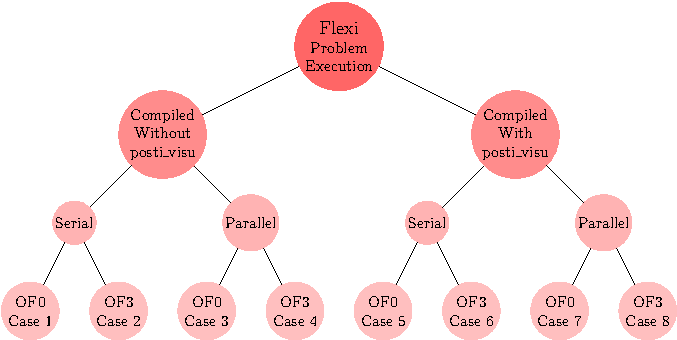
\includegraphics[width=\linewidth]{figures/chart-crop.pdf}
\caption{Output files for Flexi execution depending on the compile flag ``-DPOSTI:BOOL=ON or OFF'', the value of ''outputFile= 0  or 3`` (OF0 or OF3 in the figure), and if execution uses ``mpirun -np \#procs'' (parallel) or not (serial).  There are eight possible combinations represented by Cases 1 through 8.}
\label{fig:chart}
\end{figure}

\begingroup
\renewcommand{\labelenumi}{Case \theenumi:}
\begin{enumerate}
%Case 1
 \item Flexi is compiled with either \verb|-DPOSTI:BOOL=OFF| or omitted from the configure file, Flexi is executed in serial, and ``outputFormat = 0'' or is omitted in the parameter\_flexi.ini file.  In this case, flexi generates ONLY \verb|ProjectName_State_0*.0*.h5| files which are not readable by ParaView.

 %Case 2
 \item Flexi is compiled with either \verb|-DPOSTI:BOOL=OFF| or omitted from the configure file, Flexi is executed in serial, and ``outputFormat = 3'' in the parameter\_flexi.ini file which is the ParaView output option. This case generates the following files:
 \begin{itemize}
  \item \verb|ProjectName_State_0*.0*.h5|
  \item \verb|ProjectName_FV_0*.0*.vtu|
  \item \verb|ProjectName_DG_0*.0*.vtu|
  \item \verb|ProjectName_Solution_0*.0*.vtm|
 \end{itemize}
 \noindent The \verb|.vtm| files are readable by ParaView and has all conserved variables as well as ``FV\_Elems'' and ``IndValue'' available for display in the animation.  These last variables show how Flexi switches between Finite Volume and Discontinuous Galerkin solution methods. They are NOT available for display in ParaView if ``posti\_visu'' is used.

 %Case 3
 \item Flexi is compiled with either \verb|-DPOSTI:BOOL=OFF| or omitted from the configure file, Flexi is executed in parallel using ``mpirun -np \#processors'', and ``outputFormat = 0'' or is omitted in the parameter\_flexi.ini file. This case generates the following files:
 \begin{itemize}
  \item \verb|ProjectName_State_0*.0*.h5|
 \end{itemize}
\noindent which are NOT readable by ParaView.

%Case 4
\item Flexi is compiled with either \verb|-DPOSTI:BOOL=OFF| or omitted from the configure file, Flexi is executed in parallel using ``mpirun -np \#processors'', and ``outputFormat = 3'' in the parameter\_flexi.ini file which is the ParaView output option. This case generates the following files:
 \begin{itemize}
  \item \verb|ProjectName_State_0*.0*.h5|
  \item \verb|ProjectName_FV_0*.0*.vtu|
  \item \verb|ProjectName_DG_0*.0*.vtu|
  \item \verb|ProjectName_Solution_0*.0*.pvd|
 \end{itemize}
\noindent  The solution .pvd files are not readable by ParaView.

% Case 5
\item Flexi is compiled with \verb|-DPOSTI:BOOL=ON| in the configure file, Flexi is executed in serial and ``outputFormat = 0'' in the parameter\_flexi.ini file which is the ParaView output option. This case generates the following files:
 \begin{itemize}
  \item \verb|ProjectName_State_0*.0*.h5|
 \end{itemize}
\noindent  The solution .h5 files are not readable by ParaView. However, these h5-files are converted to ParaView readable files using posti\_visu as discussed in Section~\ref{sec:posti}.

%Case 6
\item Flexi is compiled with \verb|-DPOSTI:BOOL=ON| in the configure file, Flexi is executed in serial and ``outputFormat = 3'' in the parameter\_flexi.ini file which is the ParaView output option. This case generates the following files:
 \begin{itemize}
  \item \verb|ProjectName_FV_0*.0*.vtu|
  \item \verb|ProjectName_DG_0*.0*.vtu|
  \item \verb|ProjectName_Solution_0*.0*.vtm|
  \item \verb|ProjectName_State_0*.0*.h5|
 \end{itemize}
\noindent  The resulting solution .vtm files are readable by ParaView and displays the conserved variables as well as FV\_Elems and \verb|IndValue|.  posti\_visu is not needed in order to display these results.

% Case 7
\item Flexi is compiled with \verb|-DPOSTI:BOOL=ON| in the configure file, Flexi is executed in parallel  using ``mpirun -np \#processors'', and ``outputFormat = 0'' in the parameter\_flexi.ini file. This case generates the following files:
 \begin{itemize}
  \item \verb|ProjectName_State_0*.0*.h5|
 \end{itemize}
\noindent  The solution .h5 files are not readable by ParaView. However, these h5-files are converted to ParaView readable files using posti\_visu as discussed in Section~\ref{sec:posti}.

%Case 8
\item Flexi is compiled with \verb|-DPOSTI:BOOL=ON| in the configure file, Flexi is executed in parallel  using ``mpirun -np \#processors'', and ``outputFormat = 3'' in the parameter\_flexi.ini file which is the ParaView output option. This case generates the following files:
 \begin{itemize}
  \item \verb|ProjectName_FV_0*.0*.vtu|
  \item \verb|ProjectName_DG_0*.0*.vtu|
  \item \verb|ProjectName_Solution_0*.0*.pvd|
  \item \verb|ProjectName_State_0*.0*.h5|
 \end{itemize}
\noindent  The resulting solution .pvd files are not readable by ParaView.  However, posti\_visu will generate readable ParaView data as discussed in Section~\ref{sec:posti}.

\end{enumerate}
\endgroup
\noindent These data are summarized in Table~\ref{tab:cases}.

\begin{table}[h!]
 \centering
 \tiny
 \caption{Summary of output files generated when Flexi is executed in either serial or parallel and depending on whether or not Flexi is compiled with posti\_visu and if the outputFormat is set to either 0 or 3 in the Flexi input file. ParaView readability is noted: if ``Yes'', then all conserved variables, FV\_Elems and IndValue are available for display, if ``Yes (w/o FV\_Elems)'' means that only conserved variables are available, if ``Only discrete time pvd's'' then pvd files are readable, but only one time step at a time, while if ``NO'', ParaView gives errors when input files are read. vtm files are always readable and for all time steps so that animation is displayable in ParaView. Using posti\_visu in serial always produces vtm files, but without FV\_Elems and IndValue data.}\label{tab:cases}
 \begin{tabular}{|c|c|c|c|c|c|} \hline
  \multirow{3}{*}{Case} & -DPOSTI & Flexi: Serial(S)/Parallel(P) & Output & Solution & ParaView \\ \cline{3-3}
   & Compile & posti\_visu: Serial (S) & Format & Extensions & Readable \\
   & Flag & posti\_visu: Parallel (P)&  & & \\ \hline
% Case 1
 \multirow{3}{*}{1} & \multirow{3}{*}{OFF} & S & \multirow{3}{*}{0} & h5 & No \\ \cline{3-3} \cline{5-6}
    &  &  N/A & & N/A & N/A \\
    &  &  N/A & & N/A & N/A \\ \hline

% Case 2
 \multirow{3}{*}{2} & \multirow{3}{*}{OFF} & S & \multirow{3}{*}{3} & h5, vtu, vtm & Yes \\ \cline{3-3} \cline{5-6}
     &  &  N/A & & N/A & N/A \\
    &  &  N/A & & N/A & N/A \\ \hline

% Case 3
 \multirow{3}{*}{3} & \multirow{3}{*}{OFF} & P & \multirow{3}{*}{0} & h5 & No \\ \cline{3-3} \cline{5-6}
    &  &  N/A & & N/A & N/A \\
    &  &  N/A & & N/A & N/A \\ \hline

% Case 4
 \multirow{3}{*}{4} & \multirow{3}{*}{OFF} & P & \multirow{3}{*}{3} & h5, vtu, pvd & No \\ \cline{3-3} \cline{5-6}
   &  &  N/A & & N/A & N/A \\
    &  &  N/A & & N/A & N/A \\ \hline

% Case 5
\multirow{3}{*}{5} & \multirow{3}{*}{ON} & S & \multirow{3}{*}{0} & h5 & No \\ \cline{3-3} \cline{5-6}
    &  &  S & & vtu, vtm & Yes (w/o FV\_Elems) \\
    &  &  P & & pvtu, pvd, vtu & Only discrete time pvd's \\ \hline

% Case 6
\multirow{3}{*}{6} & \multirow{3}{*}{ON} & S & \multirow{3}{*}{3} & h5, vtu, vtm & Yes \\ \cline{3-3} \cline{5-6}
   &  &  S & & vtu, vtm & Yes (w/o FV\_Elems) \\
    &  &  P & & pvtu, pvd, vtu & Only discrete time pvd's \\ \hline

% Case 7
\multirow{3}{*}{7} & \multirow{3}{*}{ON} & P & \multirow{3}{*}{0} & h5 & No \\ \cline{3-3} \cline{5-6}
   &  &  S & & vtu, vtm &  Yes (w/o FV\_Elems) \\
    &  &  P & & pvtu, pvd, vtu & Only discrete time pvd's  \\ \hline

% Case 8
\multirow{3}{*}{8} & \multirow{3}{*}{ON} & P & \multirow{3}{*}{3} & h5, vtu, pvd & No \\ \cline{3-3} \cline{5-6}
   &  &  S & & vtu, vtm & Yes  (w/o FV\_Elems)  \\
  &   &  P & & pvtu, pvd, vtu & Only discrete time pvd's \\ \hline
 \end{tabular}
\end{table}

\subsection{posti\_visu Post Processing}\label{sec:posti}

When Flexi is finished, Paraview~[\cite{ParaView}] can be used to visualize the transient results and will require a group of \verb|.vtm| or \verb|.pvd| input files.  Flexi provides a tool called posti\_visu which converts Flexi State files to ParaView input files, which (assuming execution is in the data subdirectory mentioned above) can be generated using the command:

\begin{verbatim}
 path-to-posti_visu/posti_visu ../parameter_flexi.ini \
    ./ProjectName_State.000000*.*.h5
\end{verbatim}
\noindent for serial execution of posti\_visu or

\begin{verbatim}
 mpirun -np #processors path-to-posti_visu/posti_visu \
     ../parameter_flexi.ini ./ProjectName_State.000000*.*.h5
\end{verbatim}
\noindent for parallel execution of posti\_visu, where ''ProjectName``  is defined in the \verb|parameter_flexi.ini| file using the \verb|ProjectName =| variable.  This way of executing posti\_visu gives the default output: the conserved variables listed in Table~\ref{tab:flexiVars}.  If primitive varables are desired to be displayed either use the ParaView Calculator application discussed in Section~\ref{sec:usingParaView} or a parameter\_postiVisu.ini file can be created using the primitive variable names given in Table~\ref{tab:flexiVars} according to the directions in Section 5.10 of the Flexi Project Documentation (\textit{c.f.,} Flexi Project Documentation in the ''references`` directory) and shown in the following example:

\begin{verbatim}
nvisu = 10
varname=Density
varname=Pressure
varname=VelocityX
varname=EnergyStagnation
varname=Mach
varname=EnthalpyStagnation
\end{verbatim}

\subsection{Using ParaView}\label{sec:usingParaView}

ParaView should be already installed on your computer and available in the \verb|$PATH|-environment variable. Open paraview in the ``data'' subdirectory and load the solution \verb|.vtm| file group as shown in Figure\ref{fig:openPV} and \ref{fig:applyPV}. Because of ParaView's interpretation of the input time stamp for each .vtm file, say a tool is available (\textit{c.f.,} the \textbf{tools/makePVD/ directory}) called makepvd.py which will create a new input file with all output residing in one file.  This is particularly relevent when the final stop time for Flexi is $\ge 1.$ The dependent variables of the solution are listed in the Properties window and may be selected for transient display using the ``Solid Color'' drop-down menu above the display.  For example, selecting density and clicking on the green right-arrow button, the density is shown at each solution time step (\textit{e.g.,} Figure \ref{fig:DensityField})

% Read ParaView files
\begin{figure}
\centering
\begin{subfigure}{.95\textwidth}
  \centering
  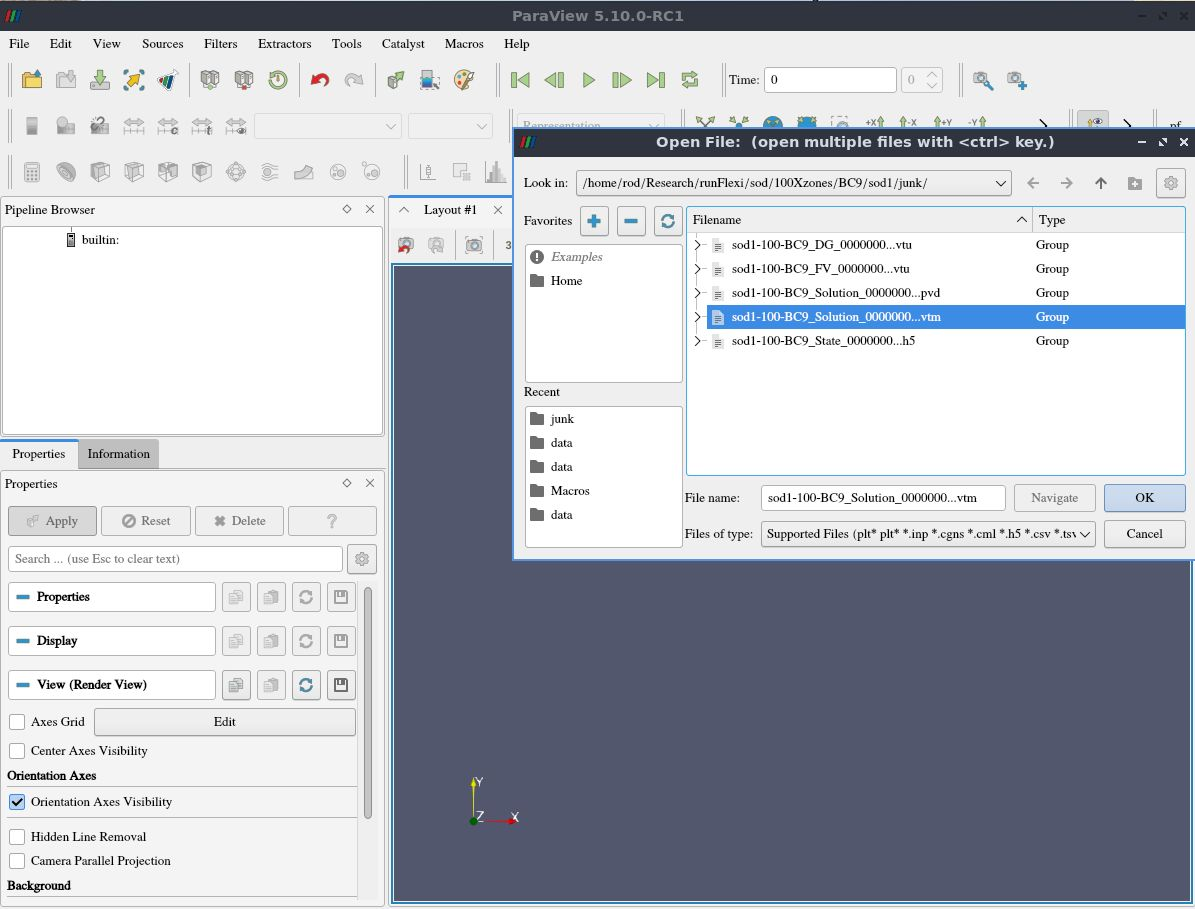
\includegraphics[width=.9\linewidth,height=0.9\linewidth,scale=1]{figures/paraviewGrabs/OpenFiles.jpg}
  \caption{Open the .vtm file group in ParaView}
  \label{fig:openPV}
\end{subfigure}
\begin{subfigure}{.95\textwidth}
  \centering
  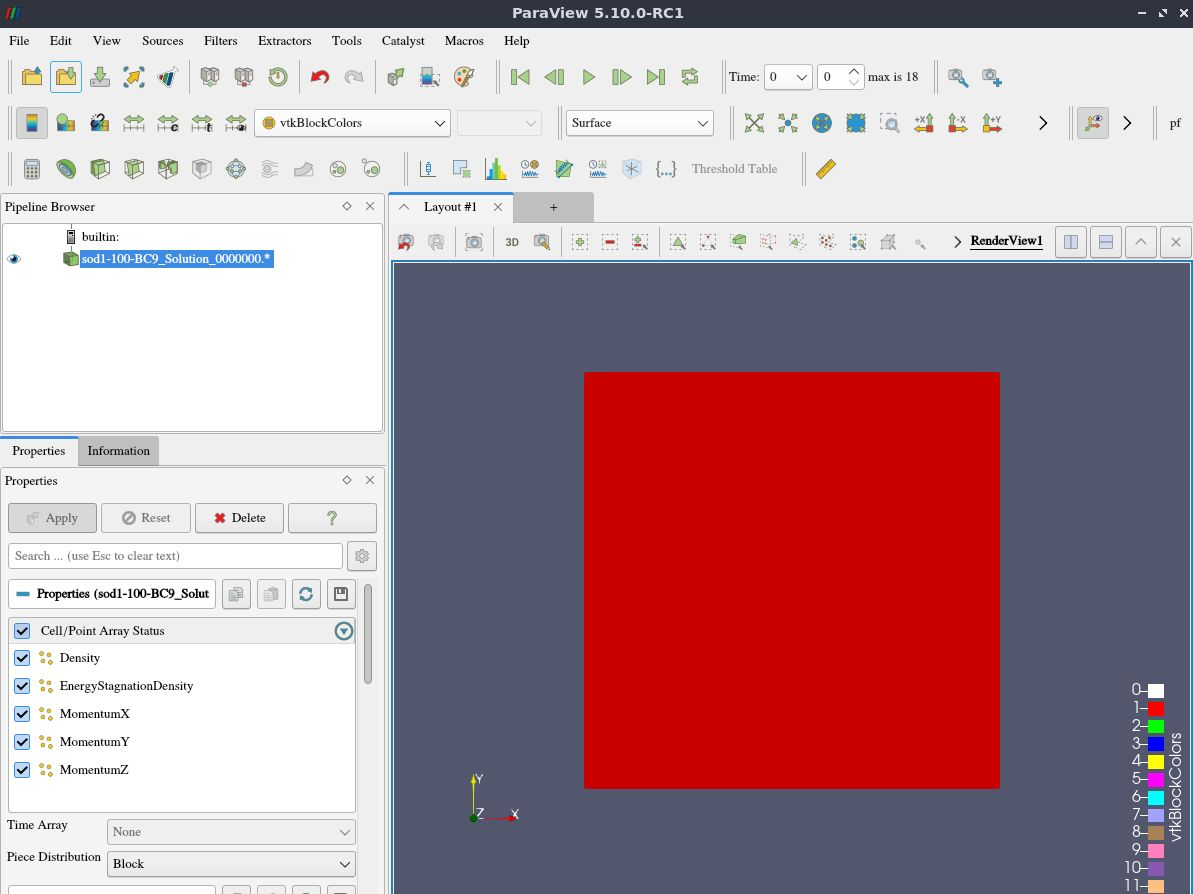
\includegraphics[width=.9\linewidth,height=0.9\linewidth,scale=1]{figures/paraviewGrabs/AfterApply-openfile.jpg}
  \caption{ParaView display after opening data files and clicking Apply in the Properties window.}
  \label{fig:applyPV}
\end{subfigure}
\end{figure}

\begin{figure}[ht]\ContinuedFloat
\centering
\begin{subfigure}{.95\textwidth}
  \centering
  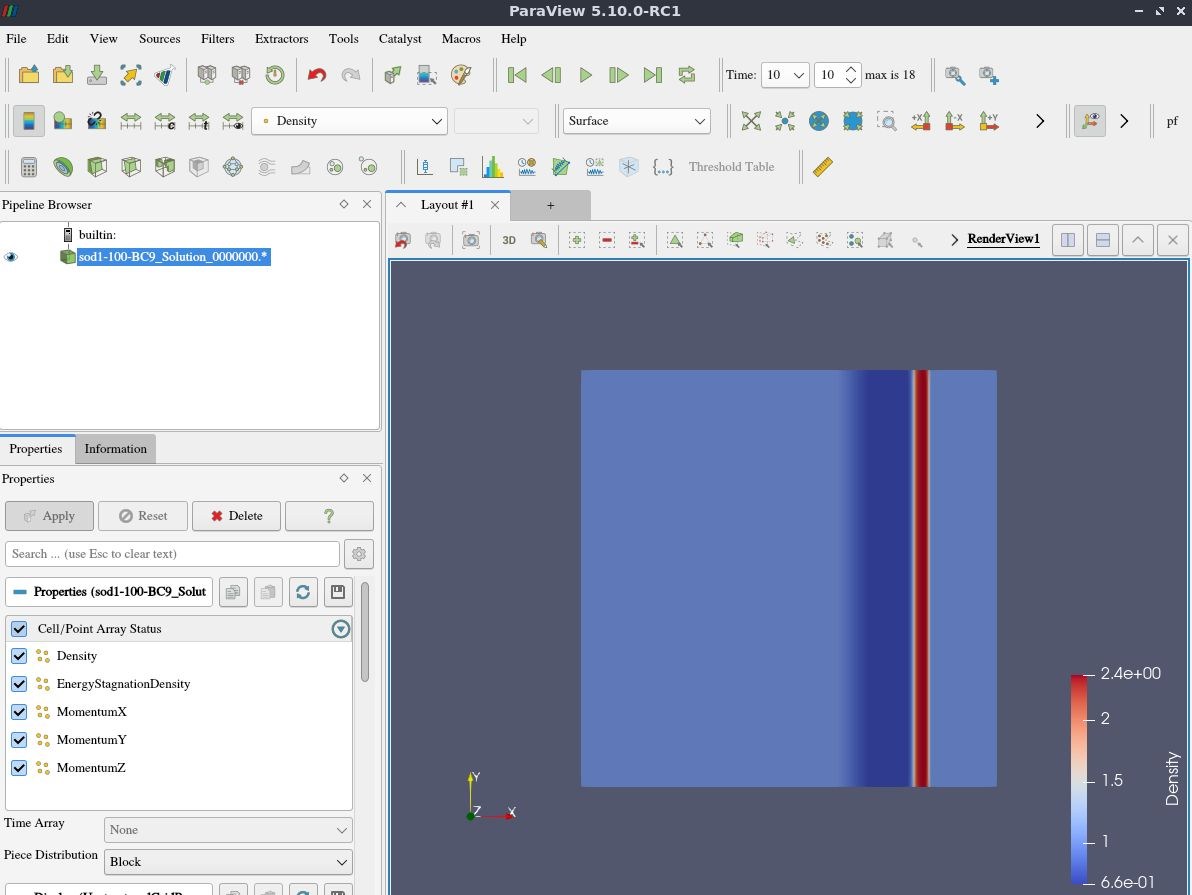
\includegraphics[width=.9\linewidth,height=0.9\linewidth,scale=1]{figures/paraviewGrabs/DensityField.jpg}
  \caption{The Density field displayed at the $10^{th}$ time step in the solution.}
  \label{fig:DensityField}
\end{subfigure}
\caption{ParaView: Reading Flexi simulation data files.}
\label{fig:PVopenFile}
\end{figure}

% Use Calculator app to create new variables

Because Flexi uses Density, MomentumX, MomentumY, MomentumZ, and EnergyStagnationDensity as the conserved solution variables primitive variables like pressure, internal energy, and x-velocity can be computed in ParaView using the Calculator application found in the Filters $\rightarrow$ Common menu located at the top line of the display.  For example, Figure \ref{fig:CalcXvel} shows that once the Calculator app is started, a new entry appears in the Pipeline Browser under the solution data and a new window opens in the Properties tab.  Either Cell or Point Data can be selected (depending on the type of data read in) and next to the ``Result Array Name'' is a box in which a new variable name is entered.  In the Figure, ``xvel'' is entered and in the next box below is entered the equation to convert ``MomentumX'' to ``xvel'' by dividing by ``Density''.  Each variable name can be either typed in or selected from the Scalars or Vectors menu at the bottom.  Clicking on Apply does the calculation and makes the new variable ``xvel'' available for plotting or use in other Calculators. Additional primitive variables are shown in Figures\ref{fig:CalcEint}, \ref{fig:CalcPres} and \ref{fig:CalcC} for specific internal energy, pressure, and sound speed, respectively.

\begin{figure}
\centering
\begin{subfigure}{.95\textwidth}
  \centering
  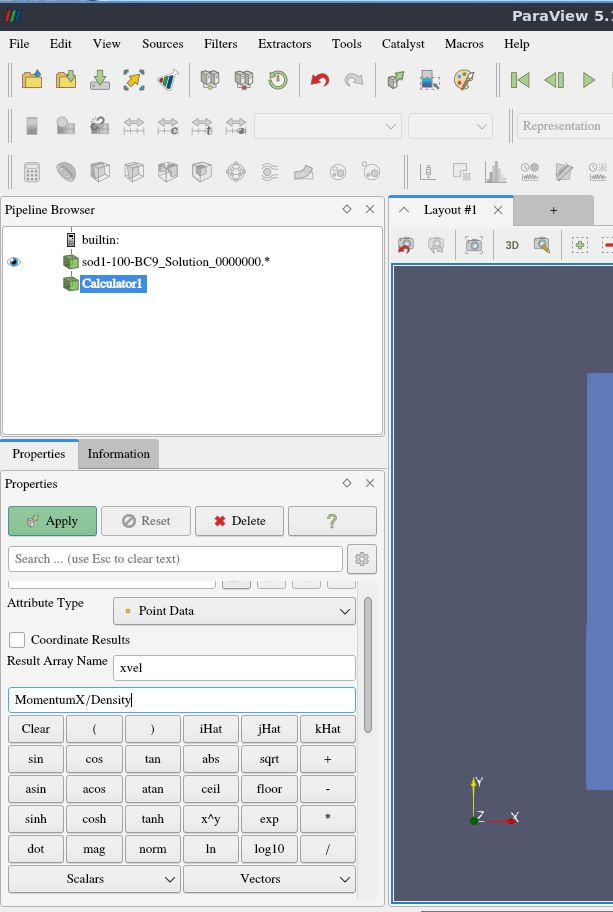
\includegraphics[width=.9\linewidth,height=0.9\linewidth,scale=1]{figures/paraviewGrabs/CalculatorXvel.jpg}
  \caption{Use the Calculator app to calculate the x-velocity.}
  \label{fig:CalcXvel}
\end{subfigure}
\begin{subfigure}{.95\textwidth}
  \centering
  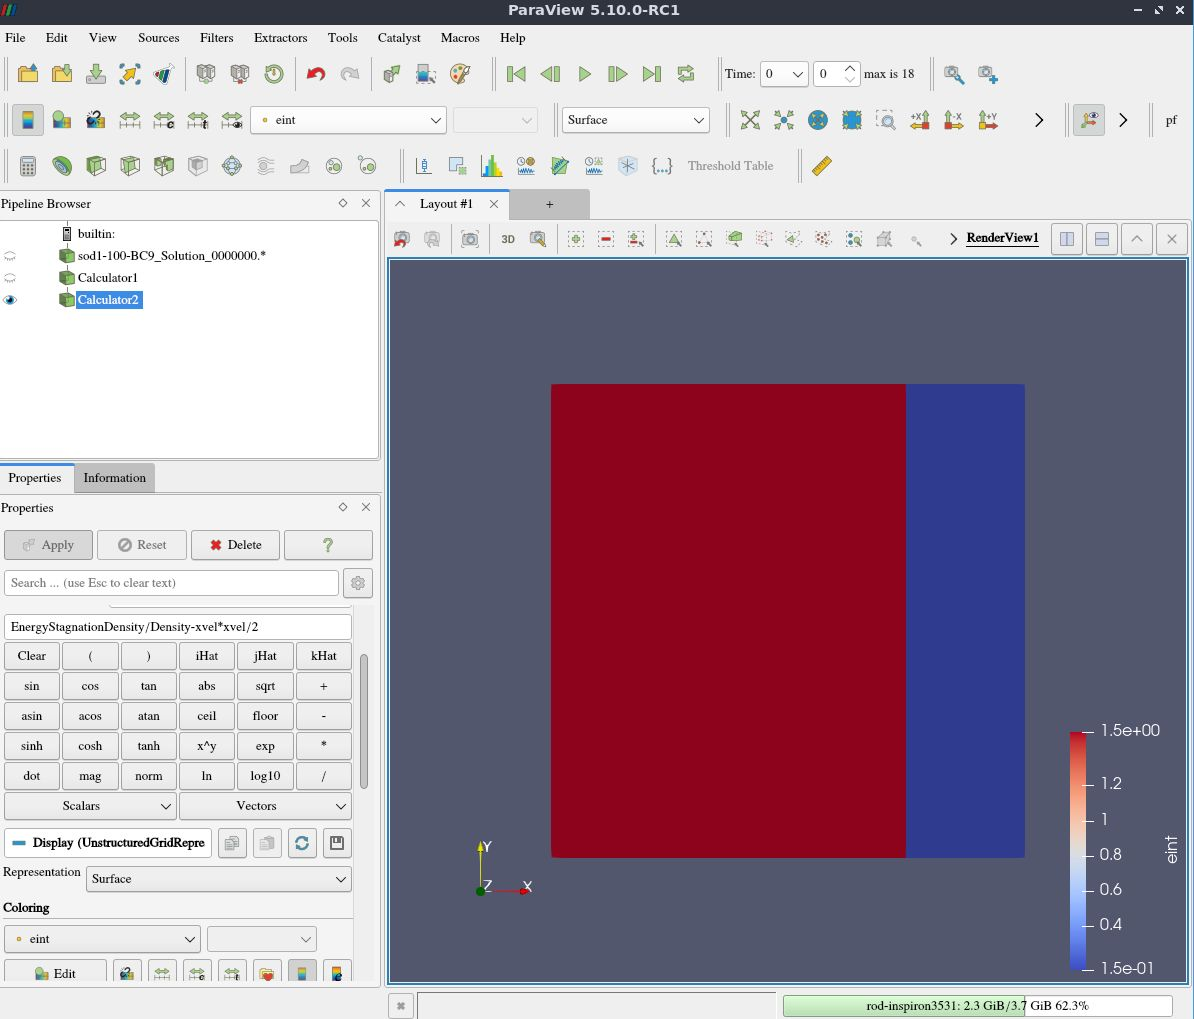
\includegraphics[width=.9\linewidth,height=0.9\linewidth,scale=1]{figures/paraviewGrabs/CalculatorEint.jpg}
  \caption{Use the Calculator app to calculate the specific internal energy.}
  \label{fig:CalcEint}
\end{subfigure}
\end{figure}

\begin{figure}\ContinuedFloat
\centering
\begin{subfigure}{.95\textwidth}
  \centering
  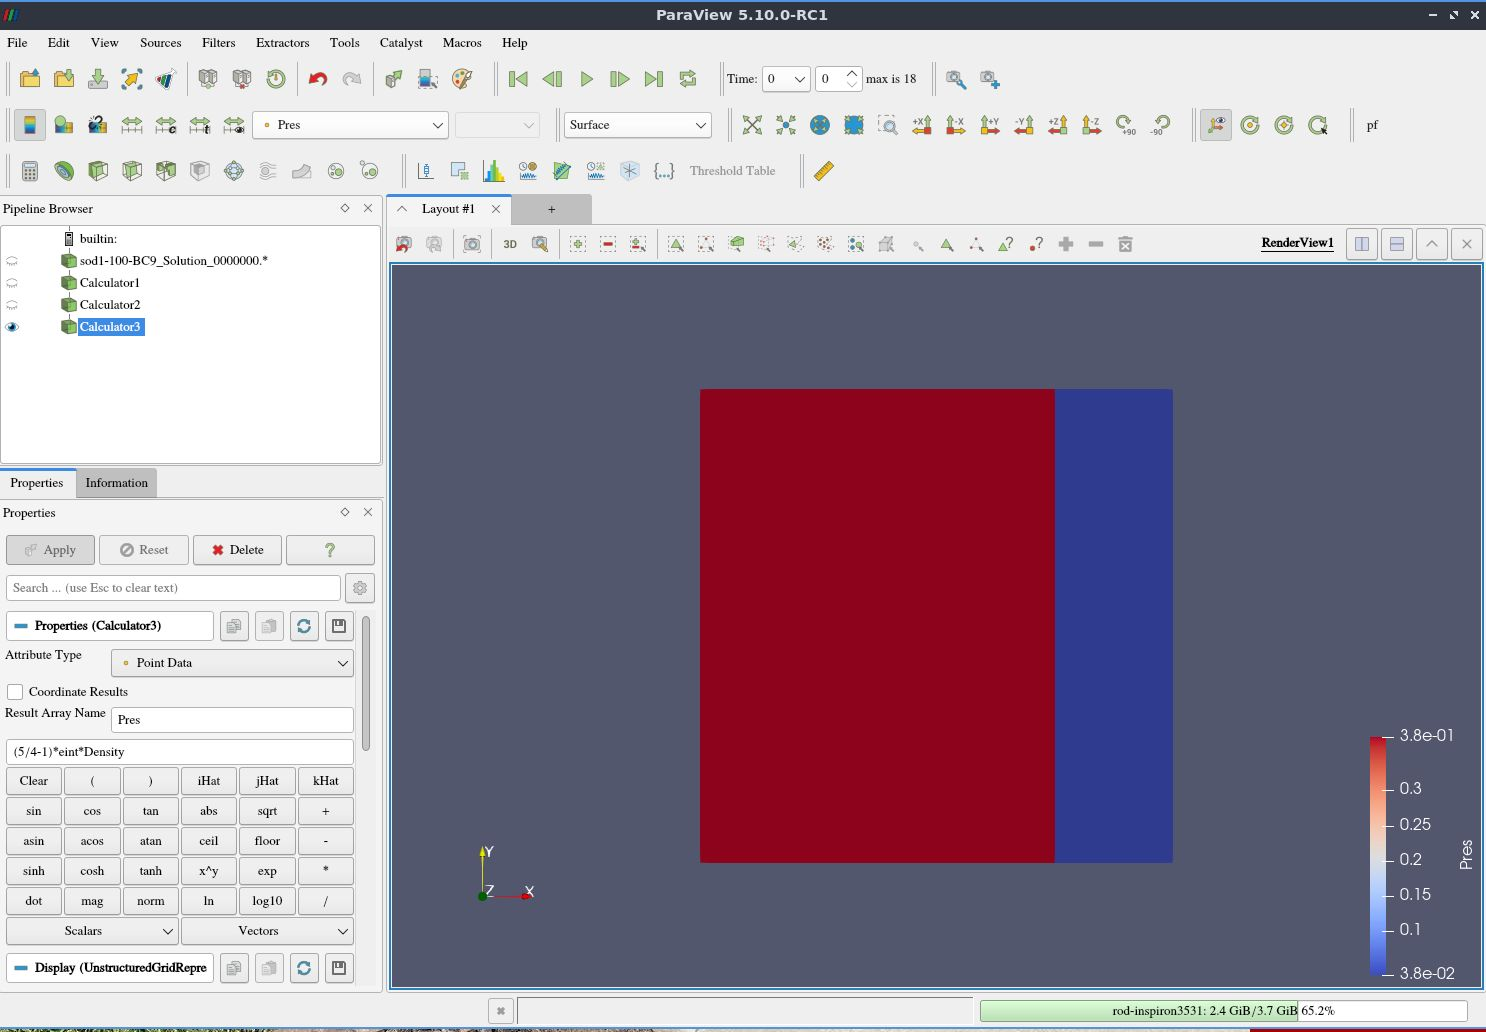
\includegraphics[width=.9\linewidth,height=0.9\linewidth,scale=1]{figures/paraviewGrabs/CalculatorPres.jpg}
  \caption{Use the Calculator app to calculate the pressure.}
  \label{fig:CalcPres}
\end{subfigure}
\begin{subfigure}{.95\textwidth}
  \centering
  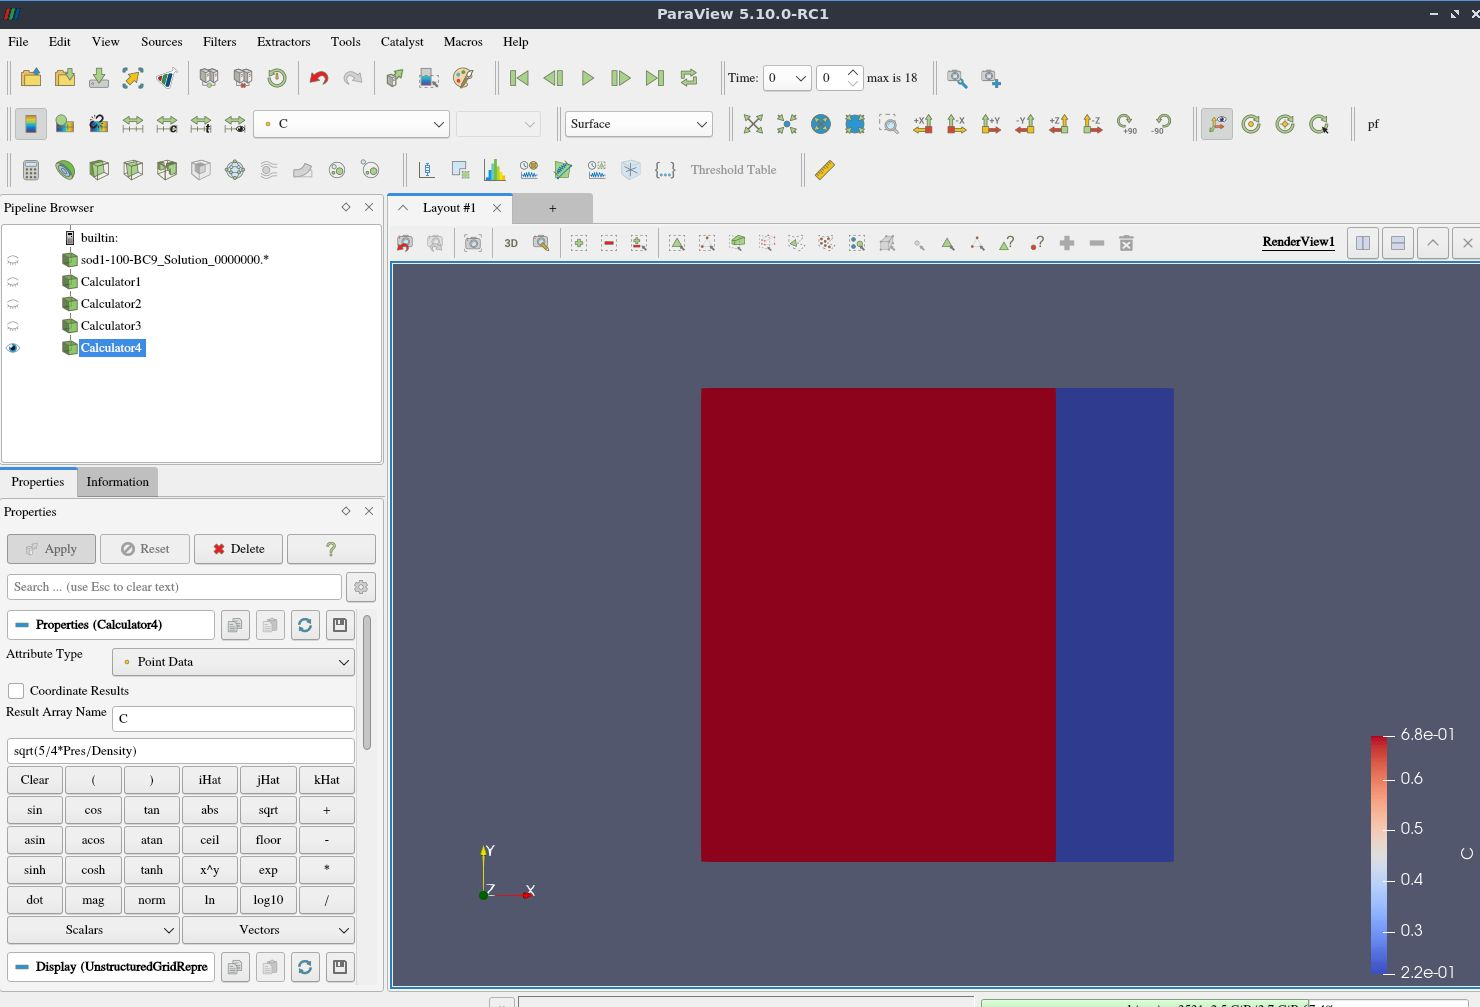
\includegraphics[width=.9\linewidth,height=0.9\linewidth,scale=1]{figures/paraviewGrabs/CalculatorC.jpg}
  \caption{Use the Calculator app to calculate the speed of sound.}
  \label{fig:CalcC}
\end{subfigure}
\caption{ParaView: Using the Calculator app to compute primative variables.}
\label{fig:CalcExamples}
\end{figure}

For one dimensional problems as computed in a three dimension mesh it is often desired to extract line plots of the dependent and/or primitive variables from ParaView displays.  In addition, the plot data may need to be exported so that the numerical data may be used for other analytical purposes.  Using the example in the prior two Figures, the following Figure\ref{fig:POL} shows a way to do these operations. Figure \ref{fig:POL1} shows the display when, from the top row of File, Edit, \textit{etc.} options, the Filters $\rightarrow$ Common $\rightarrow$ plot-over-line app is selected.  In the  ``Properties'' window along the left side under Line Parameters, adjust the Point 1 and Point 2 coordinates to be the end points of the line along which the plot is to be made.  Then click ``Apply'' resulting in the display as shown in Figure \ref{fig:POL2}. A new window called ``LineChartView 1`` opens displaying the plot of all varables available.  (The other window, ''Layout \# 1``, can be closed by clicking on the ''X`` button on the top right corner.) In the ''Properties'' window move the vertical slider nearest the Layout window dow until you see a table of potential display variables.  Select those desired for this line plot (its line color can be changed by double-clicking on the colored button next to the variable name; a new color selection window pops up from which the new color may be chosen.  When done, click on ``Apply'', resulting in a line plot as shown in Figure \ref{fig:POL3}.  To save the actual coordinate and variable data for this line plot, click on the ``File'' pull-down menu at the very top row of the display and select ``Export Scene'', resulting in a new window appearing on the display, as shown in Figure \ref{fig:POL4}.  Here, the directory for the saved data as well as its name and output type are set.  The export can be in comma-separated, tab-separated, or text data files.  If EPS, PDF, PS, or SVG are selected from the ``Files of type'' menu, the plots themselves are saved in the selected format.  When done selcting options, click on ``OK'' and except the default values in the resulting windows.

\begin{figure}
\centering
\begin{subfigure}{.95\textwidth}Asec:configFiles
  \centering
  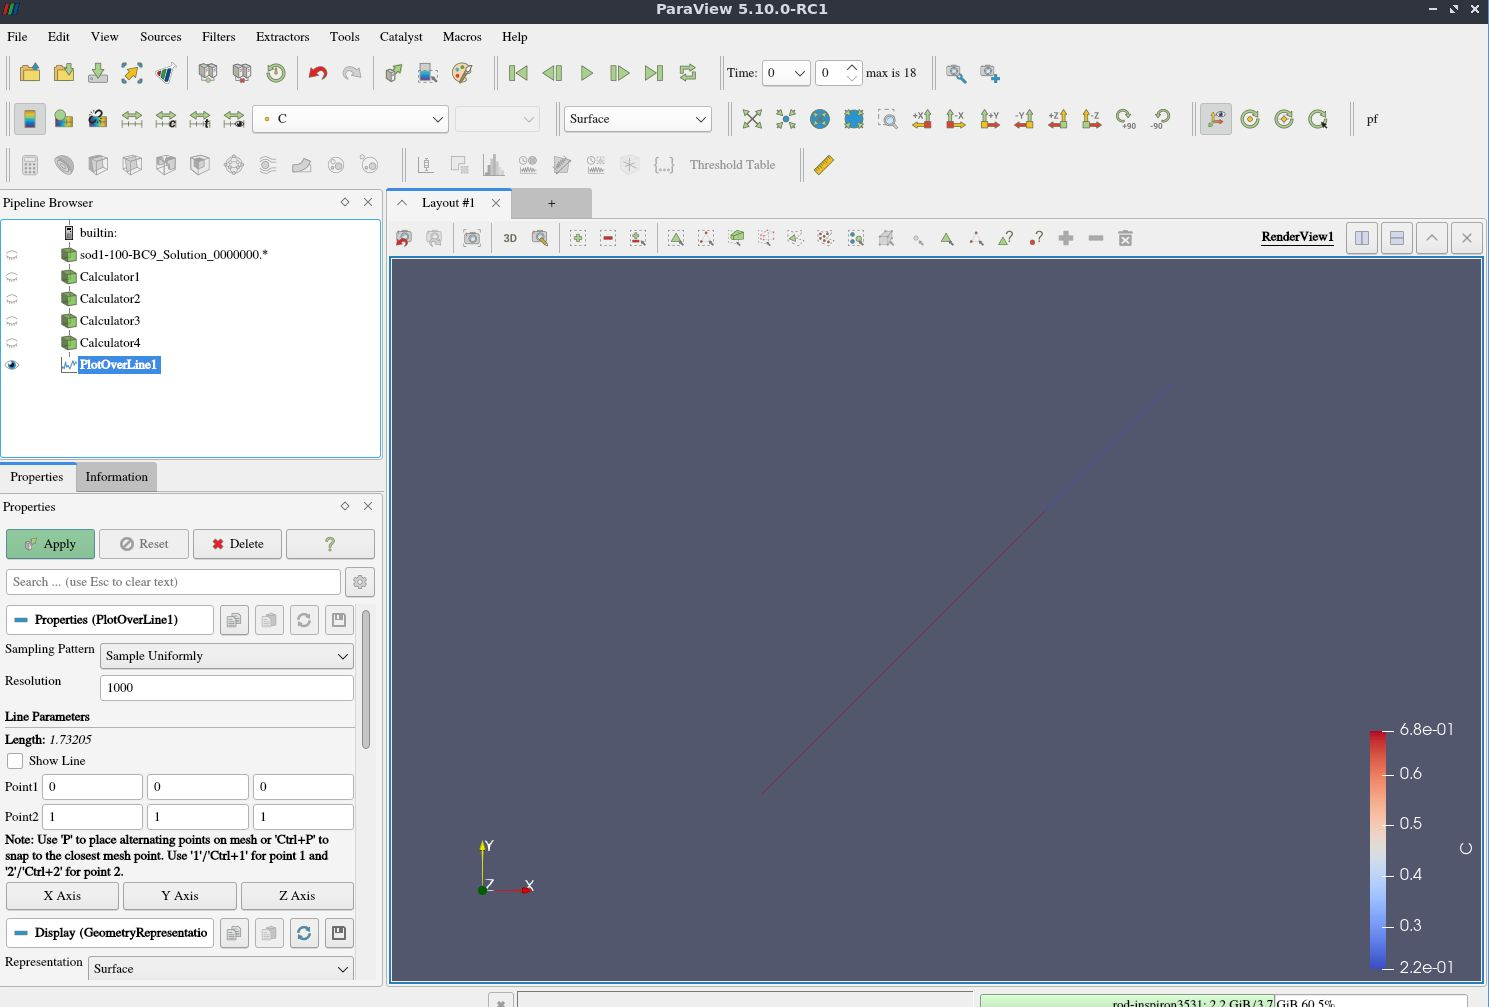
\includegraphics[width=.9\linewidth,height=0.9\linewidth,scale=1]{figures/paraviewGrabs/POL1.jpg}
  \caption{Use the Plot-Over-Line app to extract line plots of simulation data.}
  \label{fig:POL1}
\end{subfigure}
\begin{subfigure}{.95\textwidth}
  \centering
  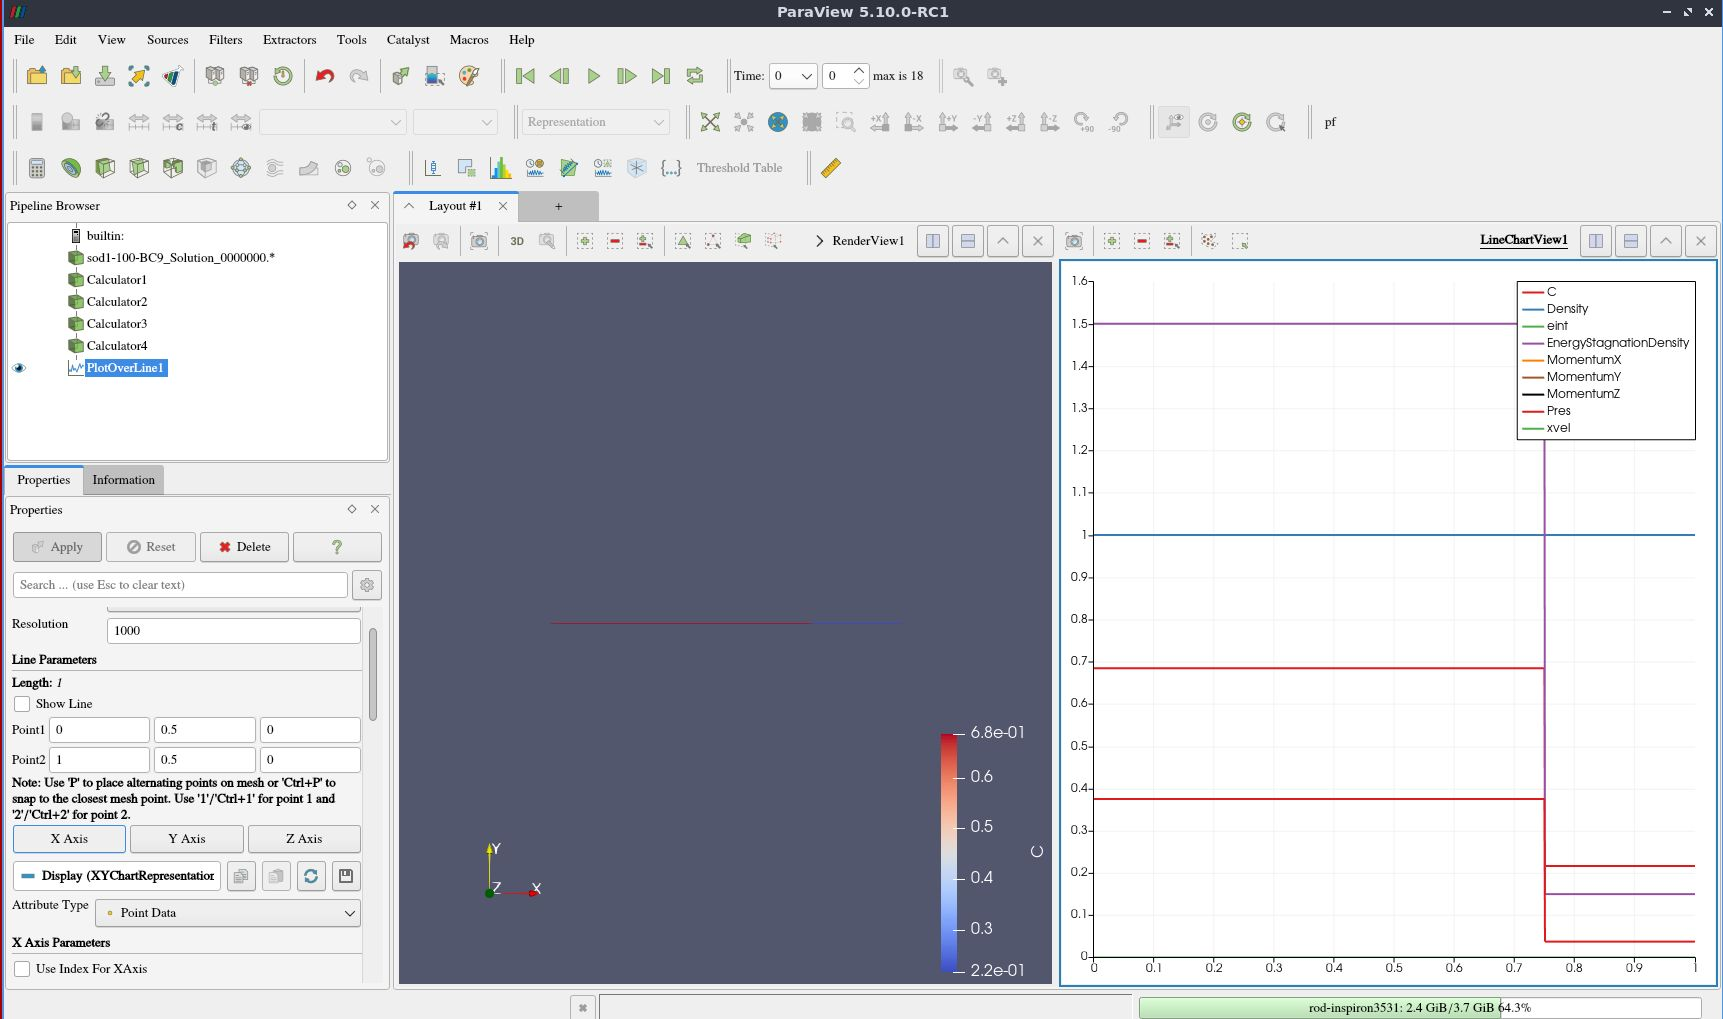
\includegraphics[width=.9\linewidth,height=0.9\linewidth,scale=1]{figures/paraviewGrabs/POL2.jpg}
  \caption{Use the Calculator app to calculate the specific internal energy.}
  \label{fig:POL2}
\end{subfigure}
\end{figure}
\begin{figure}\ContinuedFloat
\centering
\begin{subfigure}{.95\textwidth}
  \centering
  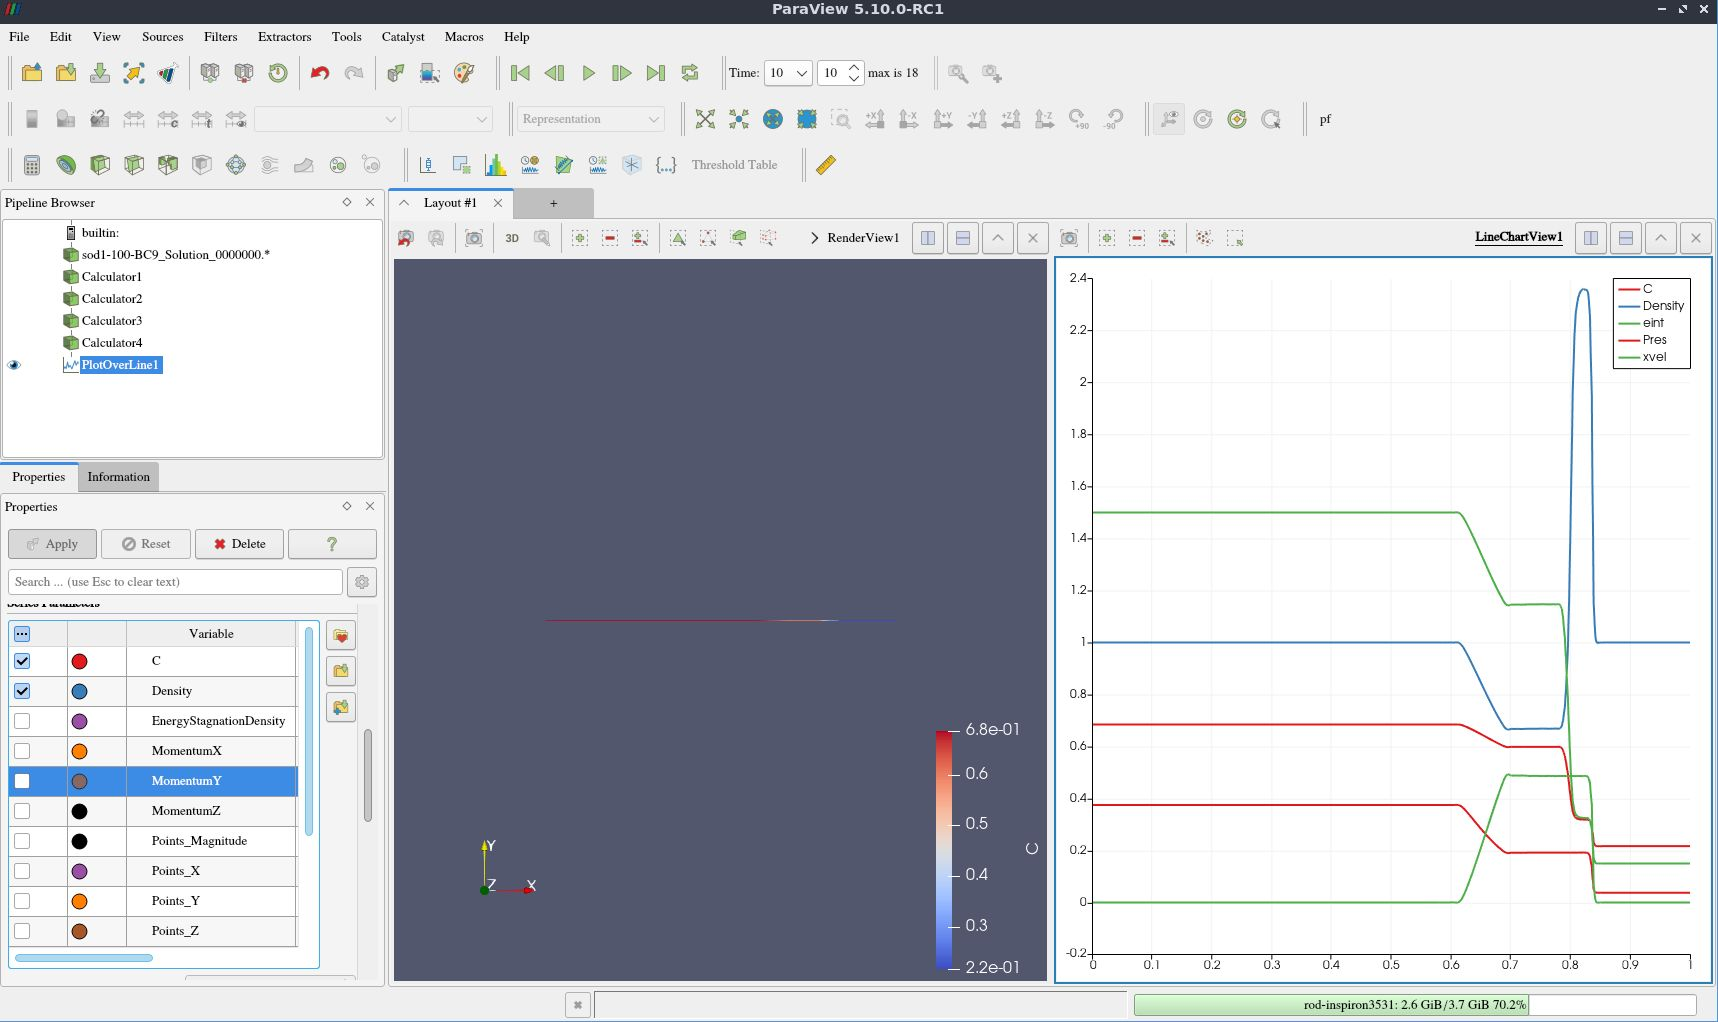
\includegraphics[width=.9\linewidth,height=0.9\linewidth,scale=1]{figures/paraviewGrabs/POL3.jpg}
  \caption{Use the Calculator app to calculate the pressure.}
  \label{fig:POL3}
\end{subfigure}
\begin{subfigure}{.95\textwidth}
  \centering
  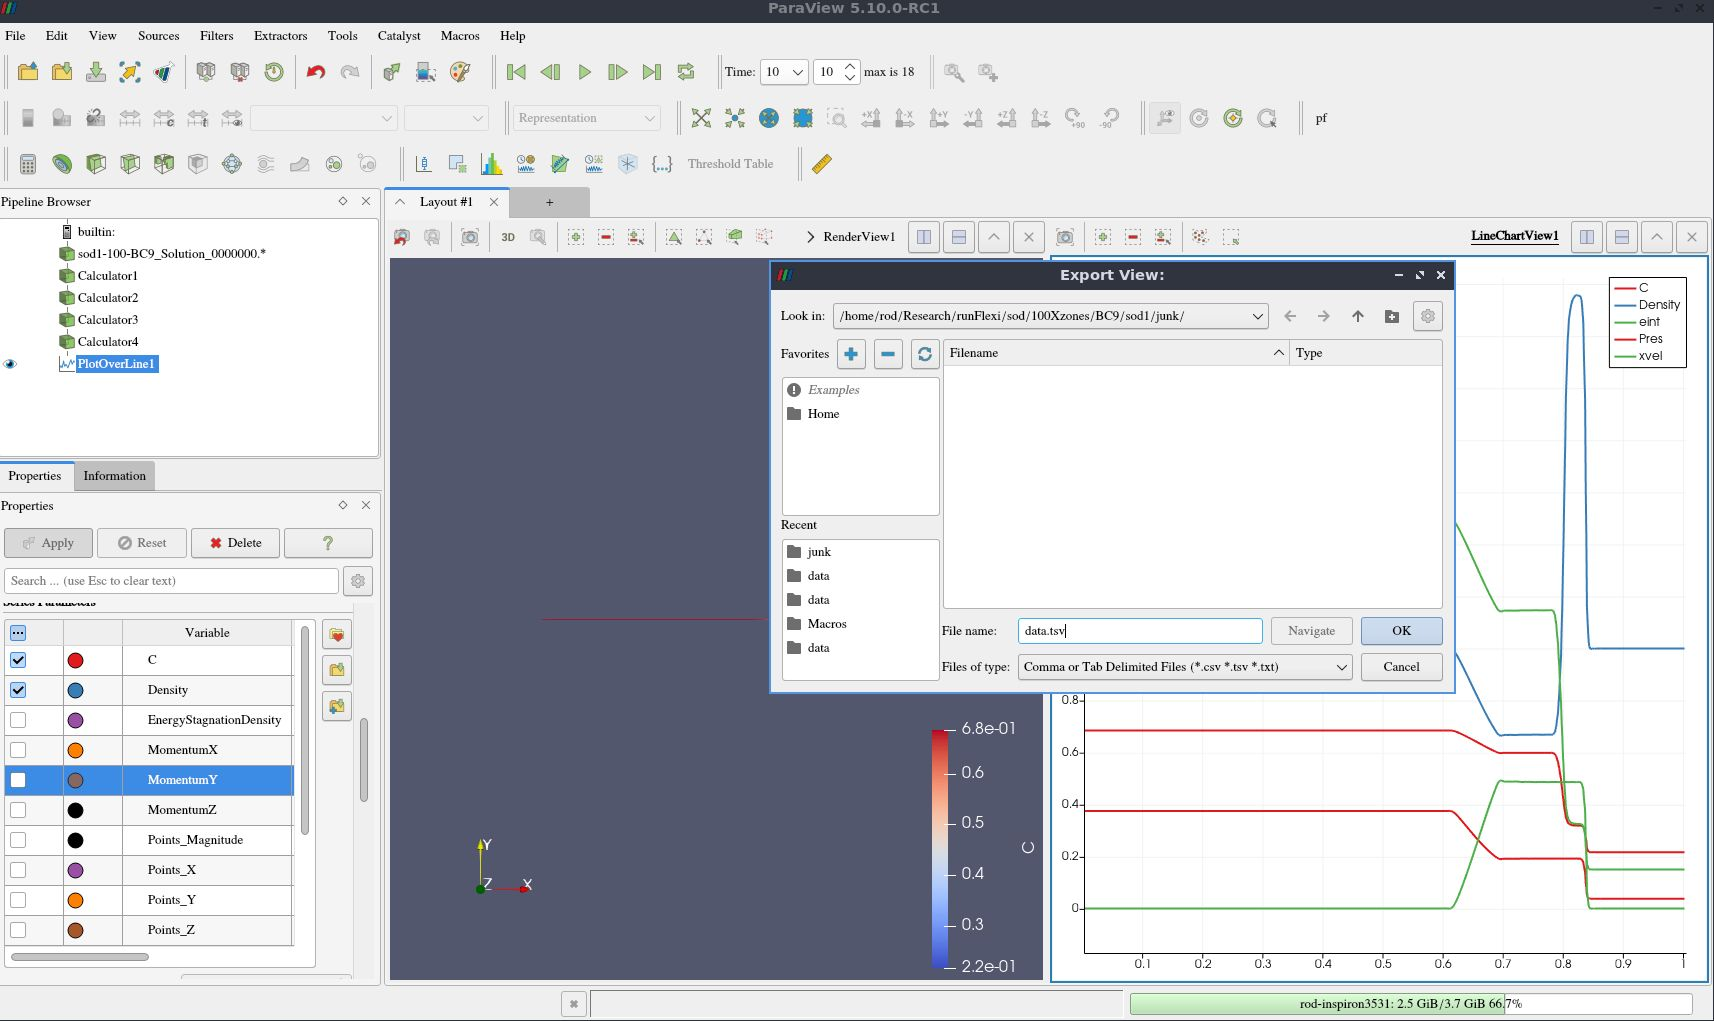
\includegraphics[width=.9\linewidth,height=0.9\linewidth,scale=1]{figures/paraviewGrabs/POL4.jpg}
  \caption{Use the Calculator app to calculate the speed of sound.}
  \label{fig:POL4}
\end{subfigure}
\caption{ParaView: Extracting line plots of simulation data and exporting numerical values for the plot data.}
\label{fig:POL}
\end{figure}

\section{Using xfig with PDF\LaTeX}\label{Asec:xfig}
\setcounter{figure}{0}

Using xfig\footnote{Using xfig version 3.2.8b with \LaTeX\  prepared using Kile version 2.9.93.  The computer operating system is Ubuntu 22.04.2 LTS} with PDF\LaTeX\  was done using the following process. Figure~\ref{fig:xfigRaw} shows a figure loaded into xfig with \LaTeX symbols  added to the figure in Text mode.  This drawing is then exported using the ''Combined PDF/\LaTeX (both parts)'' option, which generates the two files as discussed below.  The results after PDF\LaTeX processing are shown in Figure~\ref{fig:xfigLatex}.

\begin{enumerate}
 \item In xfig, create the desired drawing or load a ''.fig`` file
  \begin{enumerate}
   \item Locate on the drawing where text and/or symbols are to appear
   \item Using the \textbf{T} (TEXT input from keyboard) button,  click on the location
   where \LaTeX text is to appear.
   \item Enter the text as you would in a \LaTeX document
   \item Repeat as needed
   \item When finished with the drawing, save the figure
   \item Click on the File button and select ''export''
   \item From the ``Language'' menu select ``Combined PDF/\LaTeX (both parts)''
   \item In the ``Output file'' box, enter the file name (with the .pdf extension)
   \item In the ``Current Dir'' box, enter the  desired directory where the exported file  will be located
   \item The final figure size can be modified using the ``Magnification \%'' button
   \item Finally, click on the ``Export'' button on the bottom of the window
   \item xfig will ask if you want to save the figure.
   \item Answers ``Yes'' or ``No'' will result in 2 files being written to disk: \verb|outFileName.pdftex_t| and \verb|outFileName.pdftex|
  \end{enumerate}
\item In the document being prepared, create a figure environment (with centering if desired).  For example:

\begin{verbatim}
\begin{figure}[ht]
 \begin{center}
  \input{figures/shocktube.pdftex_t}
  \caption{Sod shock tube initial conditions.}
  \label{fig:shockICs}
 \end{center}
\end{figure}
\end{verbatim}

\noindent Note that the input file has the  ``pdftex\_t'' extension and is editable.  It contains the \verb|\includegraphics{shocktube.pdftex}| command and should be modified to give its correct path, in this case \\ \verb|\includegraphics{figures/shocktube.pdftex}|.
\end{enumerate}

\begin{figure}[h!]
\centering
\begin{subfigure}[h!]{\linewidth}
\centering
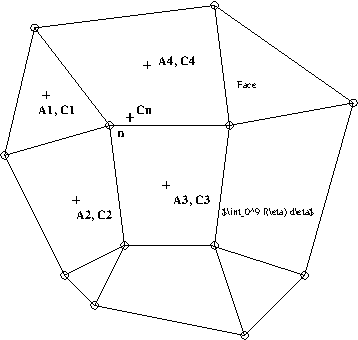
\includegraphics[scale=1.]{figures/CentPDF.pdf}
\caption{Using \LaTeX commands in xfig figure.}
  \label{fig:xfigRaw}
\end{subfigure}

\bigskip

\begin{subfigure}[h!]{\linewidth}
\centering
\input{figures/centLA.pdf_t}
\caption{\LaTeX processed figure.}
\label{fig:xfigLatex}
\end{subfigure}%
\caption{Using xfig with PDF\LaTeX.}
\end{figure}

\section{Flexi Input Files}\label{Asec:flexiinput}

\subsection{$\mathrm{sod}_1$ parameter\_flexi.ini File}\label{ssec:flexiin-sod1}
\verbatiminput{inputFiles/parameter_flexi-sod1.ini}

\subsection{$\mathrm{sod}_2$ Flexi Input: Free Boundaries}\label{ssec:flexiin-sod2-BC2}
\verbatiminput{inputFiles/parameter_flexi-sod2-BC2.ini}

\subsection{$\mathrm{sod}_2$ Flexi Input: Symmetry Boundaries}\label{ssec:flexiin-sod2-BC9}
\verbatiminput{inputFiles/parameter_flexi-sod2-BC9.ini}

\subsection{$\mathrm{sod}_3$ Flexi Input: Free Boundaries}\label{ssec:flexiin-sod3-BC9}
\verbatiminput{inputFiles/parameter_flexi-sod3-BC9.ini}

\subsection{Einfeldt 123-Problem Flexi Input}\label{ssec:flexiin-einfeldt}
\verbatiminput{inputFiles/parameter_flexi-einfeldt.ini}

\subsection{LeBlanc-Problem Flexi Input}\label{ssec:flexiin-leblanc}
\verbatiminput{inputFiles/parameter_flexi-leblanc.ini}

\subsection{Sedov-Problem Flexi Input}\label{ssec:flexiin-sedov}
\verbatiminput{inputFiles/parameter_flexi-sedov.ini}

\subsection{Hui Problem ($\beta = 0$) Flexi Input}\label{ssec:flexiin-hui-Rot0}
\verbatiminput{inputFiles/parameter_flexi-hui-Rot0.ini}

\subsection{Hui Problem ($\beta = 0.4$) Flexi Input}\label{ssec:flexiin-hui-Rot}
\verbatiminput{inputFiles/parameter_flexi-hui-Rot.ini}


\section{HOPR Input Files}\label{Asec:hoprinput}

\subsection{$\mathrm{sod}_1$ HOPR Input}\label{ssec:hoprin-sod1}
\verbatiminput{inputFiles/parameter_hopr-sod1.ini}

\subsection{$\mathrm{sod}_2$ HOPR Input: Inflow/Outflow Boundaries}\label{ssec:hoprin-sod2-BC2}
\verbatiminput{inputFiles/parameter_hopr-sod2-BC2.ini}

\subsection{$\mathrm{sod}_2$ HOPR Input: Symmetry Boundaries}\label{ssec:hoprin-sod2-BC9}
\verbatiminput{inputFiles/parameter_hopr-sod2-BC9.ini}

\subsection{$\mathrm{sod}_3$ HOPR Input: Inflow/Outflow Boundaries}\label{ssec:hoprin-sod3-BC9}
\verbatiminput{inputFiles/parameter_hopr-sod3-BC9.ini}

\subsection{Einfeldt 123-problem HOPR Input: Inflow/Outflow Boundaries}\label{ssec:hoprin-einfeldt}
\verbatiminput{inputFiles/parameter_hopr-einfeldt.ini}

\subsection{LeBlanc Problem HOPR Input}\label{ssec:hoprin-leblanc}
\verbatiminput{inputFiles/parameter_hopr-leblanc.ini}

\subsection{Sedov-Problem HOPR Input}\label{ssec:hoprin-sedov}
\verbatiminput{inputFiles/parameter_hopr-sedov.ini}

\subsection{Hui Problem ($\beta = 0$) HOPR Input}\label{ssec:hoprin-hui-Rot0}
\verbatiminput{inputFiles/parameter_hopr-hui-Rot0.ini}

\subsection{Hui Problem ($\beta = 0.4$) HOPR Input}\label{ssec:hoprin-hui-Rot}
\verbatiminput{inputFiles/parameter_hopr-hui-Rot.ini}

\end{appendices}
